\documentclass[12pt,german]{article}

\usepackage[left=2cm, right=2cm, top=2cm, bottom=3.5cm, landscape=false]{geometry}

\usepackage{graphicx}
\usepackage{float}

\usepackage{tabularx}
\newcolumntype{R}{>{\raggedleft\arraybackslash}X}
\newcolumntype{L}{>{\raggedright\arraybackslash}X}
\newcolumntype{C}{>{\centering\arraybackslash}X}
\usepackage{booktabs}
\usepackage{dcolumn}

\usepackage[ngerman]{babel}

\usepackage{amsmath}

\title{\vspace{-1.5cm}Protokoll Gammadosisleistung}
\author{Fuchs, Gutmann, Kosbab, Kowal, Steindorf, Fälker, Richter}

\begin{document}
    \maketitle
    \tableofcontents

    \section{Kurzbeschreibung des Versuches}
    \begin{itemize}
        \item 
    \end{itemize}

    \section{Nullwertmessungen}
    \begin{table}[H]
        \begin{tabularx}{\textwidth}{R|R|R}
            \toprule
            \raggedright\textbf{Messung} & \raggedright\textbf{Messwert ohne Menschen} & \multicolumn{1}{l}{\textbf{Messwert mit Menschen}} \\
            & $[Bq]$ & $[Bq]$ \\
            \midrule
            1 & 522 & 408 \\
            2 & 522 & 488 \\
            3 & 545 & 415 \\
            4 & 526 & 396 \\
            5 & 575 & 492 \\
            \midrule
            \O & $N_0$ = 538 & 439,8 \\
            \bottomrule
        \end{tabularx}
        \caption{Untergrundstrahlung bei laufendem Reaktor mit und ohne Menschen als Abschirmmaterial}
    \end{table}

    \section{Messwerte}
    \begin{table}[H]
        \begin{tabularx}{\textwidth}{L|R|R|R|R|R|R}
            \toprule
            \textbf{Zeit} & \multicolumn{2}{c|}{\textbf{Al: $[Bq]$}} & \multicolumn{2}{c|}{\textbf{Cu: $[Bq]$}} & \multicolumn{2}{c}{\textbf{X: $[Bq]$}} \\
            $[min]$ & \multicolumn{1}{c}{$N_i$} & \multicolumn{1}{c|}{$N_i - N_0$} & \multicolumn{1}{c}{$N_i$} & \multicolumn{1}{c|}{$N_i - N_0$} & \multicolumn{1}{c}{$N_i$}$N_i$ & \multicolumn{1}{c}{$N_i - N_0$} \\
            \midrule
            0 & - & - & - & - & - & -   \\
            0,5 & 24505 & 23967 & 24063 & 23525 & 11971 & 11433   \\
            1,0 & 21163 & 20625 & 22350 & 21812 & 11134 & 10596   \\
            1,5 & 18339 & 17801 & 20668 & 20130 & 10651 & 10113   \\
            2,0 & 15840 & 15302 & 19868 & 19330 & 10252 & 10113   \\
            2,5 & 13718 & 13180 & 18376 & 17838 & 9285  & 8747    \\
            3,0 & 11656 & 11118 & 17582 & 17044 & 8809  & 8271    \\
            3,5 & 10279 & 9741  & 16477 & 15939 & 8314  & 7776    \\
            4,0 & 8744  & 8206  & 15461 & 14923 & 8117  & 7579    \\
            4,5 & 7612  & 7074  & 14629 & 14097 & 7423  & 6885    \\
            5,0 & 6536  & 5998  & 13838 & 13300 & 7081  & 6543    \\
            5,5 & 5961  & 5423  & 12893 & 12355 & 6791  & 6253    \\
            6,0 & 5102  & 4564  & 12004 & 11466 & 6380  & 5842    \\
            6,5 & 4426  & 3888  & 11673 & 11135 & 6026  & 5488    \\
            7,0 & 3948  & 3410  & 11196 & 10658 & 5638  & 5100    \\
            7,5 & 3381  & 2843  & 10355 & 9817  & 5410  & 4872    \\
            8,0 & 3060  & 2522  & 10077 & 9539  & 5180  & 4642    \\
            8,5 & 2691  & 2153  & 9477  & 8939  & 4852  & 4314    \\
            9,0 & 2300  & 1762  & 9009  & 8471  & 4645  & 4107    \\
            10,0 & 1930 & 1392  & 8152  & 7614   & 4096  & 3558   \\
            \bottomrule
        \end{tabularx}
        \caption{Messwerte zu Zerfällen}
    \end{table}

    \section{Graphische Darstellung}
    \begin{figure}[H]
        \centering
        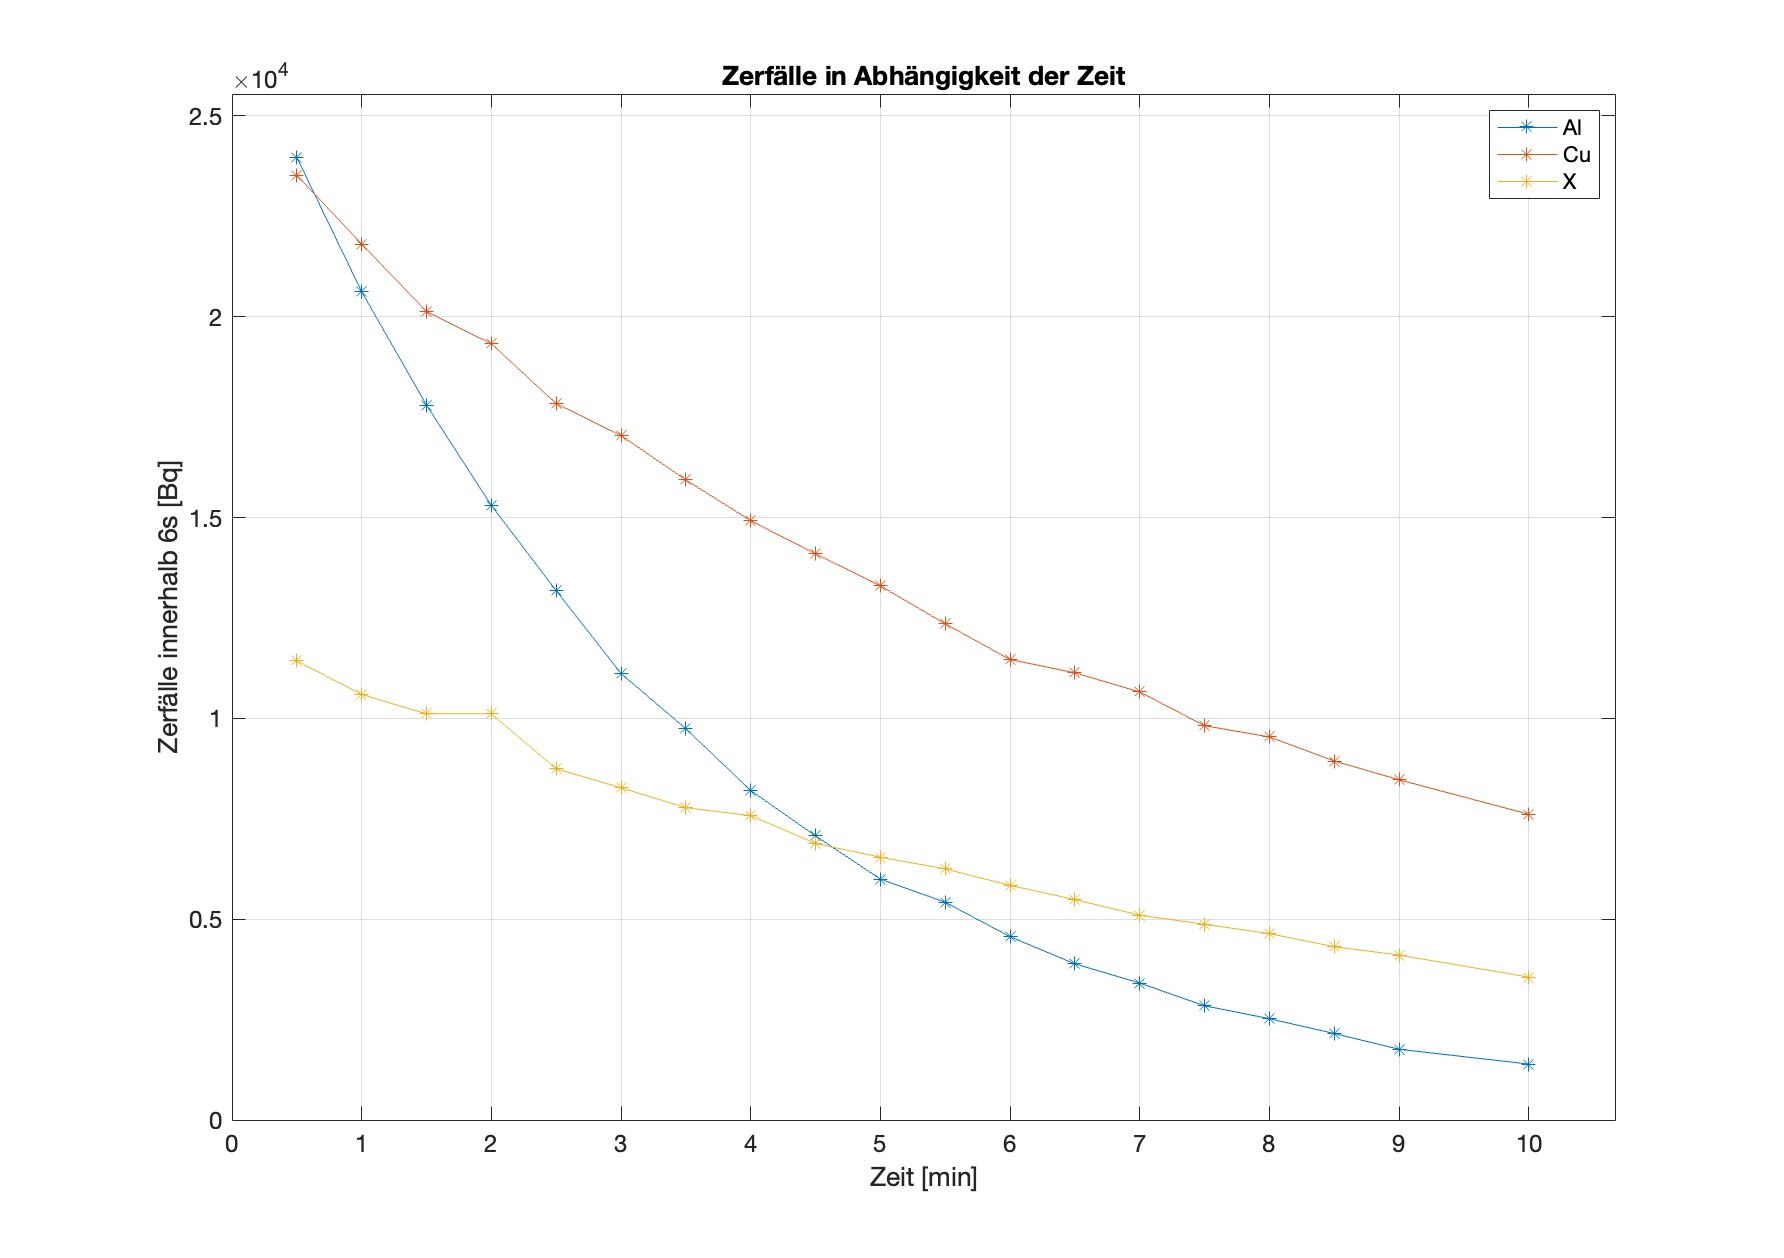
\includegraphics[width=\textwidth]{Diagramm.png}
        \caption{Messwerte mit linearer Achse}
    \end{figure}
    \begin{figure}[H]
        \centering
        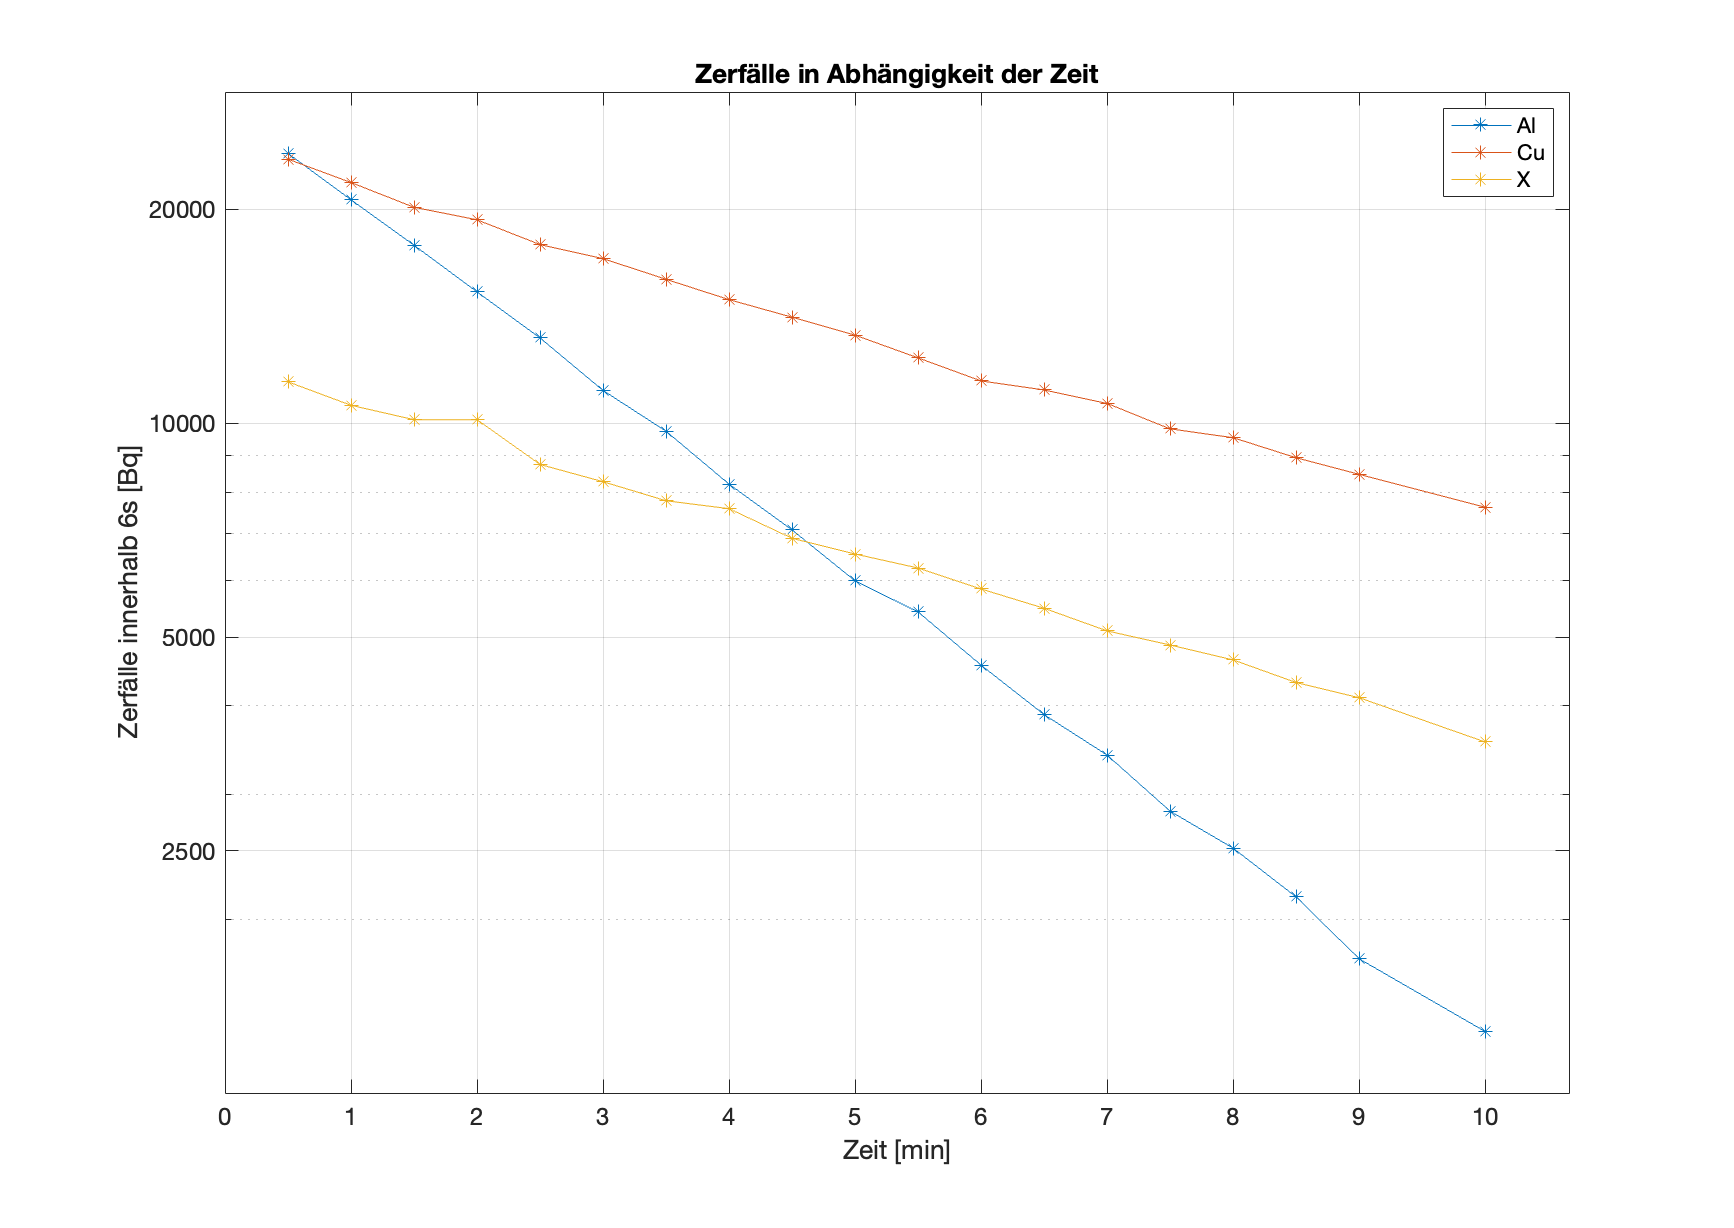
\includegraphics[width=\textwidth]{DiagrammLog.png}
        \caption{Messwerte mit logarithmischer Achse}
    \end{figure}
\end{document}